\documentclass{article}
\usepackage{amsmath} % For mathematical symbols and align environment
\usepackage{graphicx} % For including images
\usepackage{caption} % For better captions

\begin{document}

\section*{A3(b)}

To analyze the effect of regularization on polynomial regression, we first fit a polynomial of degree \( d = 8 \) with no regularization (\( \lambda = 0 \)). The resulting plot is shown in Figure \ref{fig:before_reg}. Next, we increase the regularization parameter to \( \lambda = 1 \), which penalizes large coefficients and smooths the curve. The resulting plot is shown in Figure \ref{fig:after_reg}. Increasing regularization reduces overfitting, resulting in a smoother function that generalizes better to new data points.

\begin{figure}
    \centering
    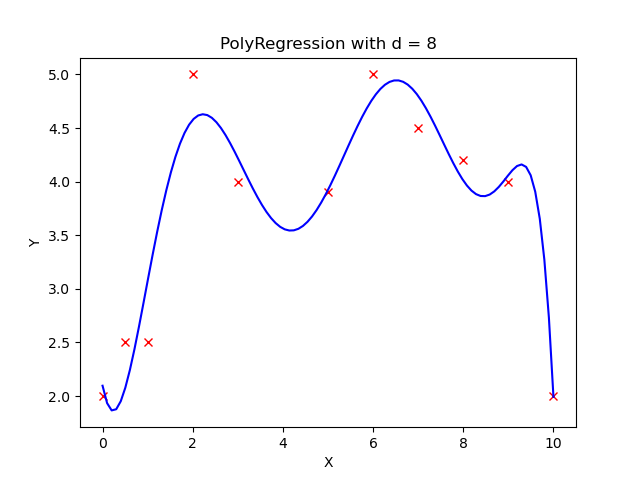
\includegraphics[width=0.5\linewidth]{C:/Users/admin/Downloads/ML/hw1/hw1/plot1_normal.png}
    \caption{Plot before increase in regularization (\( \lambda = 0 \))}
    \label{fig:before_reg}
\end{figure}

\begin{figure}
    \centering
    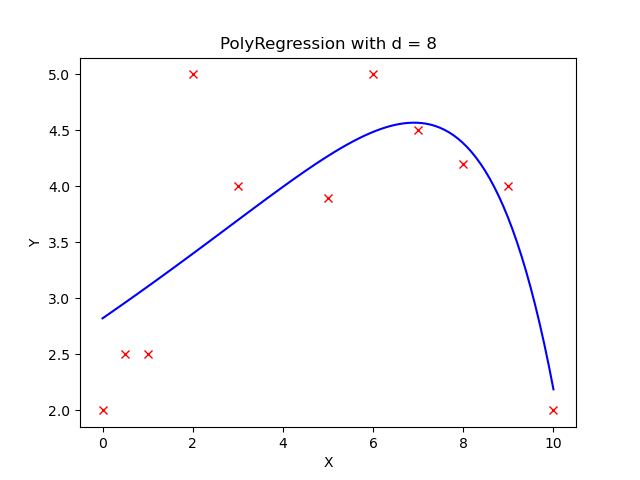
\includegraphics[width=0.5\linewidth]{C:/Users/admin/Downloads/ML/hw1/hw1/plot1_moreReg.png}
    \caption{Plot after increase in regularization (\( \lambda = 1 \))}
    \label{fig:after_reg}
\end{figure}

\end{document}
